\chapter{补充更多细节}
对于一些不宜放在正文中的重要支撑材料,可编入毕业论文的附录中。包括某些重要的原始数据、详细数学推导、程序全文及其说明、复杂的图表、设计图纸等一系列需要补充提供的说明材料。如果毕业设计(论文)中引用的实例、数据资料,实验结果等符号较多时,为了节约篇幅,便于读者查阅,可以编写一个符号说明,注明符号代表的意义。附录的篇幅不宜太多,一般不超过正文。

\section{附录里的图}

图 \ref{figA1} 显示……,图 \ref{subfigA1} 表明……。

\subsection{单张图片}
\begin{figure}[h]
	\centering
	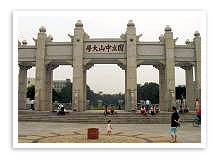
\includegraphics[width=0.8\textwidth]{figure/fig1.png}
	\caption{标题} 
	\label{figA1}
\end{figure}

\subsection{多张子图}
\begin{figure}[h!] % image examples & compare
	\begin{subfigure}{0.55\textwidth}
		\centering
		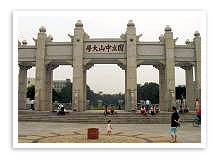
\includegraphics[width=0.5\textwidth]{figure/fig1.png}
		\caption{子图1}
		\label{subfigA1}
	\end{subfigure}
	\begin{subfigure}{0.55\textwidth}
		\centering
		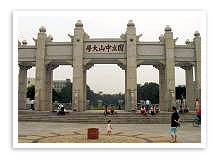
\includegraphics[width=0.5\textwidth]{figure/fig1.png} 
		\caption{子图2}
		\label{subfigA2}
	\end{subfigure}
	\begin{subfigure}{0.55\textwidth}
		\centering
		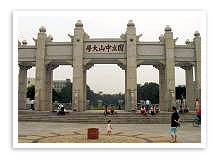
\includegraphics[width=0.5\textwidth]{figure/fig1.png}
		\caption{子图3}
		\label{subfigA3}
	\end{subfigure}
	\begin{subfigure}{0.55\textwidth}
		\centering
		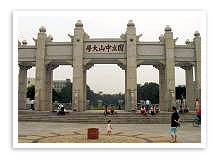
\includegraphics[width=0.5\textwidth]{figure/fig1.png} 
		\caption{子图4}
		\label{subfigA4}
	\end{subfigure}
	\caption{多子图}
	\label{subfigA}
\end{figure}




\section{附录里的表格}
表 \ref{tabA1} 表示……。
\begin{table}[h]
	\centering
	\caption{国际单位制中具有专门名称的导出单位}		
	\label{tabA1}
	\begin{tabular}{c|c|c|c}
		\toprule[2pt]
		量的名称 & 单位名称 & 单位符号 & 其他表示式例\\
		\midrule[2pt]
		频率	& 赫[兹]	& Hz	&$s^{-1}$ \\
		\hline                                        %细横线
		力;重力 	& 牛[顿]	& $N$	 & $kg·m/s^2$ \\
		\hline                                         %细横线
		压力,压强;应力	& 帕[斯卡]	&$Pa$	&$N/m^2$ \\
		\bottomrule[2pt]
	\end{tabular}
\end{table}

\section{附录里的公式}
\label{sec:formula}
\begin{equation}
\label{eqA1}
\textbf{H} = \begin{bmatrix}
I*\bm {x}_i \\ \textbf{h}
\end{bmatrix}
\end{equation}

\endinput
